\documentclass[11pt,spanish]{article}

\usepackage[a6paper, landscape,
	left=1cm, top=1cm, right=1cm, bottom=1.5cm
]{geometry}
%\usepackage[a4paper, margin=3cm]{geometry}
\usepackage{babel}
\usepackage{xltxtra}
\usepackage{grid-system}
\usepackage{multicol} % simpler than grid for lots of cases
\usepackage{hyperref}
\usepackage{xcolor}
\usepackage{graphicx}
\usepackage[export]{adjustbox}
\usepackage{fancyhdr}
\usepackage{listings}

\setmainfont{Comic Sans MS}
%\setmathfont{eulervm}
%\lstset{basicstyle=\footnotesize\ttfamily}
\lstset{basicstyle=\footnotesize\setmainfont{DejaVu Sans Mono}}

\definecolor{verletblue}{HTML}{487AD8}
\definecolor{verletgreen}{HTML}{37DE88}
\definecolor{verletcyan}{HTML}{1AFBFF}

\fancyhead{}
\fancyfoot{}
\fancyfoot[RO]{{\footnotesize \thepage\ de\ \pageref*{lastpage}}}
\renewcommand{\headrule}{}
%\renewcommand{\footrule}{\vbox to 0pt{\hbox to\headwidth{\dotfill}\vss}}
% XXX should find way to use only one right aligned rule...
\renewcommand{\footrule}{{\footnotesize \rule{\textwidth - 5ex}{0pt}\rule{5ex}{1pt}\vss}}
\pagestyle{fancy}

\newcommand{\fr}[1]{%
	\begin{flushright}
		#1
	\end{flushright}
}
%row space
\newcommand{\rowsp}[1][1em]{\vspace{#1}}
\newcommand{\hone}[1]{{\rowsp[0.3em]\noindent\Large #1 \rowsp[0.3em]}}
\newcommand{\htwo}[1]{{\rowsp\noindent\large #1 \rowsp}}
\newcommand{\htworuler}[1]{{%
	\rowsp\noindent\Large #1%
	\\ {\color{verletgreen}\noindent\rule{\textwidth + 2em}{0.5em}}\rowsp%
}}
\newcommand{\hthree}[1]{{\rowsp\noindent\large #1 \rowsp[0.5em]}}
\newcommand{\hfour}[1]{{\rowsp\large #1 \rowsp[0.5em]}}
\newcommand{\for}[1]{{#1 \rowsp}}
\newcommand{\signline}{\rule{\textwidth}{1pt}}
\newcommand{\emptycell}[1][1]{\begin{Cell}{#1}\ \end{Cell}}

%=======================
% specific to presentations
%\newcommand{\myitm}{aoeuaeou}
\newcommand{\myitm}[1]{\begin{itemize}#1\end{itemize}}

\newcommand{\mydesc}[1]{%
	\begin{description}
	\setlength\itemsep{0em}%
	#1
	\end{description}
}
\newcommand{\pros}{\item[pros:]}
\newcommand{\cons}{\item[cons:]}

\setlength{\parindent}{0pt}
\setlength{\parskip}{1ex plus 0.5ex minus 0.2ex}
%=======================

%\renewcommand{\emph}[1]{\emph{#1}}

\title{Pros y contras de OpenBSD}
\author{Abel Camarillo $<$acamari@verlet.org$>$}


\begin{document}

\maketitle
\thispagestyle{empty}

\begin{center}

\includegraphics[height=0.3\textheight]{img/puflogh}
\end{center}


\newpage

\hone{Agenda}

\myitm{
	\item ¿Quién soy?
	\item ¿Qué es OpenBSD?
	\item Pros y contras
}

\newpage %===============
\hone{¿Quién soy?}
\begin{Row}
\begin{Cell}{2}
\myitm{
	\item Desarrollador de software desde el 2008 - OpenBSD, perl, C, sh, js
	\item Lead developer en Neuroservices Communications durante 6 años.
	\item Desarrollador freelance desde el 2015 - Verlet.
	\item Maintainer de 21 paquetes en el árbol oficial de OpenBSD -
	\href{http://openports.se/bbmaint.php?maint=acamari@verlet.org}{
	      http://openports.se/bbmaint.php?\textbackslash{} maint=acamari@verlet.org}
	\item Interés en UNIX, poesía, $\sim$arte$\sim$ (performance), cocina, etc...
}
\end{Cell}

\begin{Cell}{1}
\ \\ %XXX so image hasn't its bottom to baseline
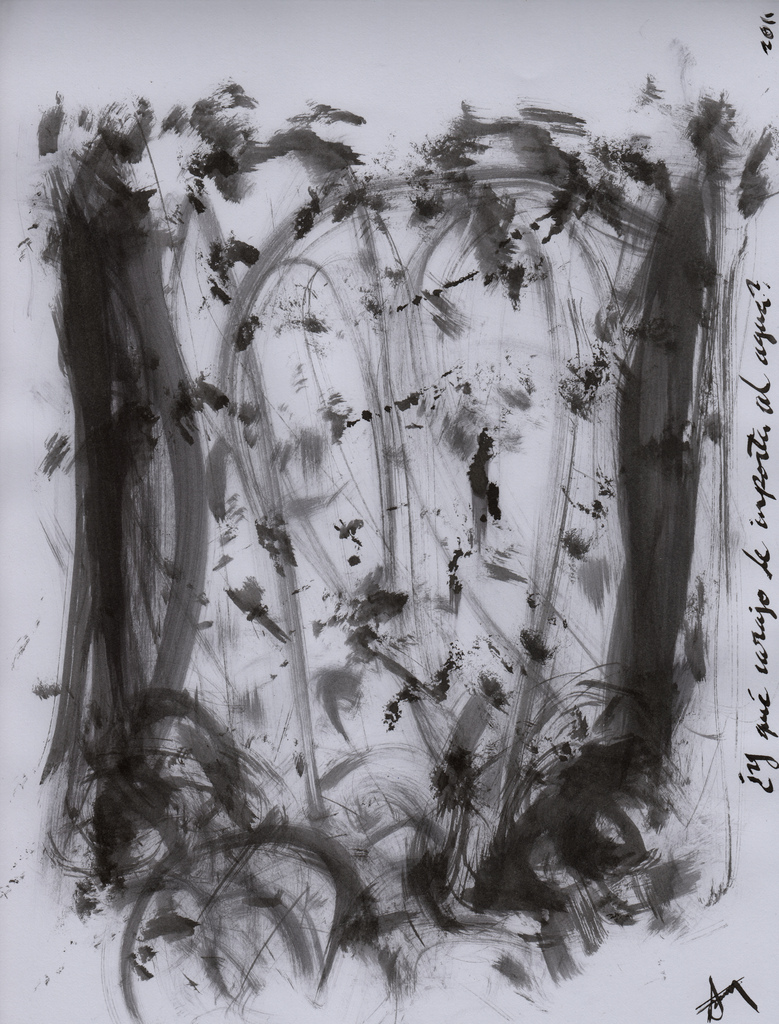
\includegraphics[width=\textwidth]{img/carajo}
\fr{ {\tiny ¿Y qué carajo\\
le importa al agua? - 2011} }
\end{Cell}

\end{Row}

\newpage %===============

\hone{¿Qué es OpenBSD?}

\begin{center}
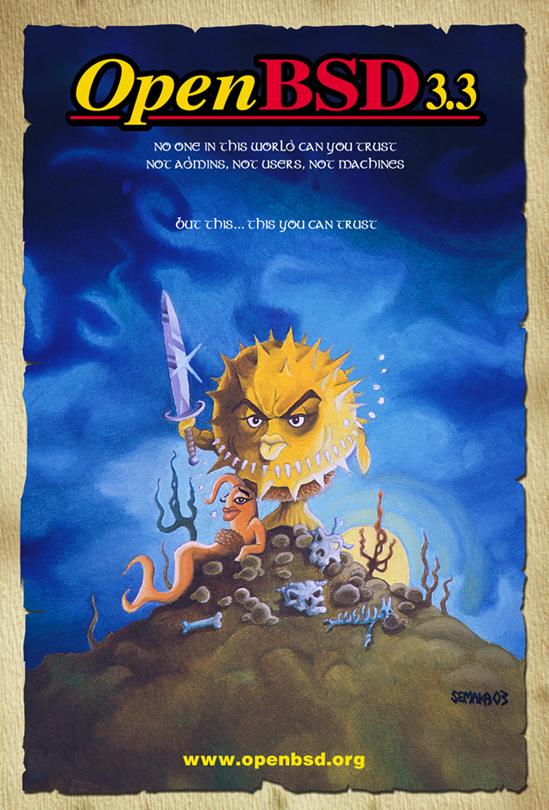
\includegraphics[height=0.81\textheight]{img/poster33}
\end{center}

\newpage %===============

\hone{Pros y contras}

\begin{multicols}{2}
\myitm{
	\pros licencia ISC, no GPLv3
	\cons no GPLv3

	\pros no docker
	\cons no docker

	\pros no blobs, no NDA
	\cons no blobs, no NDA

	\columnbreak

	\pros rolling release + release (6 meses)
	\cons n/a

	\pros openbsd pf, no iptables, no nftables
	\cons no iptables, no nftables

	\pros carp, no vrrp
	\cons no vrrp

	\pros no systemd
	\cons no systemd

	\newpage
	\pros openssh, libressl, openntpd, opensmtpd, openbsd httpd, openbsd
		dhclient, openbgpd, openbsd ospfd, ...
	\cons n/a

	\pros rolas, posters, cds
	\cons n/a

	\pros ports, binary packages
	\cons n/a

	\pros amd64, i386, sparc64, sparc, zaurus, arm* , ...
	\cons amd64, i386, sparc64, sparc, zaurus, arm*, ...

	\columnbreak
	\pros GHC, haskell
	\cons GHC, haskell

	\pros openbsd vmm, guest: xen guest (pvh), hyperv, kvm
	\cons no KVM, qemu unaccel, no xen host
}
\end{multicols}

\newpage %===============
\ 
\vspace{\stretch{1}}
\begin{center}
\hone{¿Preguntas?}
\end{center}
\vspace{\stretch{1}}

\newpage %===============
\ 
\vspace{\stretch{1}}
\begin{center}
\hone{Gracias}
\end{center}
\vspace{\stretch{1}}

\label{lastpage}
\end{document}
